	\newif\ifshowinternal
\showinternaltrue %flag for showing/hiding owners of chapters/sections... Use \showinternaltrue or \showinternalfalse. The toc may not respond immediately (~> clear cache files)
% !TeX spellcheck = en_US
\documentclass[a4paper, % DIN A4 Format
	12pt, %Schriftgröße
	%twoside, %zweiseitiges Layout (linke und rechte Seiten)
	%openright, %Kapitel fangen immer auf rechter Seite an
	cleardoublepage=empty, %evtl. eingefügte Seiten sind leer (ohne Seitenzahl), alternativ: cleardoublepage=plain (mit Seitenzahl)
	numbers=noenddot, %hinter Kapitel- und Abschnittsnummern grundsätzlich kein Punkt am Ende
	BCOR1.5cm
	]{scrbook} % Dokumentklasse aus KOMA-Paket, alternativ: scrartcl oder scrreprt
\usepackage[utf8]{inputenc}
\usepackage{cite}
\usepackage[hidelinks]{hyperref} %Jan: I hope this does not cause problems again. Just remove the [hidelinks] parameter if it does.
\usepackage{listings}
\usepackage[pdftex]{graphicx}
\usepackage[\ifshowinternal \else disable\fi]{todonotes}
\usepackage{enumerate}
\usepackage{longtable}
\usepackage{float}

%for fancy table stuff
\usepackage{xcolor} 
\usepackage{colortbl}
\usepackage{multicol} 
\usepackage{booktabs}
\usepackage{multirow}
\usepackage{rotating}
\usepackage{tabularx}


\usepackage{latexsym,multicol,color,pstricks}
\usepackage{listings} % comes with texlive−latex−recomended
\lstdefinelanguage{Uppaal}{ % syntax highlight via font
basicstyle=\small\sffamily, % small sans−serif font (like verdana)
keywords={after update,assign,before update,break,case,const,continue,
default,else,enum,for,guard,if,meta,process,progress,return,select,
state,sync,switch,trans,system,while},
keywords={[2]broadcast,bool,clock,chan,commit,init,int,scalar,struct,
typedef,urgent,void}, keywordstyle={[2]\bfseries},
keywords={[3]false,true}, otherkeywords={[3]−>},
morekeywords={[3]−>}, keywordstyle={[3]\bfseries},
comment=[l]{//}, morecomment=[s]{/∗}{∗/}, % single and multi−line
commentstyle=\itshape, % appear in italic
tabsize=4, % tab treatment (going to be fixed in Uppaal)
captionpos=b, % put captions at the bottom
escapechar=@ % write LaTeX comments escaped by @ symbol
}
\lstdefinelanguage[GUI]{Uppaal}[]{Uppaal}{ % syntax like in GUI
keywordstyle={[2]\color{black!50!green}}, % slightly darker than in GUI
otherkeywords={−>}, keywordstyle={[3]\color{magenta}},
commentstyle={\color{black!50!red}\itshape}, % dark red
literate={{−−>}{$−−>$}3} % fix arrows
}
\lstdefinelanguage[LIT]{Uppaal}[GUI]{Uppaal}{ % replace some symbols
literate={{−>}{{$\leadsto$} }2 {−−>}{{$\longrightarrow$} }2
{=}{{$\gets$ }}2 {==}{{$==$}}2 {:=}{{$\gets$ }}2 {<=}{{$\leq$ }}2
{>=}{{$\geq$ }}2 {&&}{{$\land$}}2 {||}{{$\lor$}}2 {<>}{{$\Diamond$}}1
{[]}{{$\Box$}}1 {forall}{{$\forall$}}1 {exists}{{$\exists$}}1}
}

\lstnewenvironment{lstuppaal}[2]{\lstset{language={Uppaal}, 
columns={[l]flexible},
frameround=fftt, frame=shadowbox, rulesepcolor=\color{gray},
caption={#2}, label=#1}}{} %listing definition for Uppaal. Command: \begin{lstuppaal}{label}{caption}

% --- Macros ---
\usepackage{xspace}
\newcommand{\muml}{\textsc{MechatronicUML}\xspace}
\newcommand{\uppaal}{\textsc{Uppaal}\xspace}
\newcommand{\fujaba}{\textsc{FujabaRT-Suite}\xspace}
\newcommand{\cybertron}{\textsc{Cybertron}\xspace}
\newcommand{\rtsc}{\textsc{Real-Time Statechart}\xspace}
\newcommand{\pCCI}{passive continuous component instance} %it's in another file so we can easily migrate macro changes between theses. 
\newcommand{\titleinfo}{Overtaking with approacher} 
\title{\titleinfo}
%\subtitle{} % no subtitle. 
\author{} %TODO


\begin{document}

\thispagestyle{empty}
\begin{titlepage}
	\begin{center}
	  

	  \begin{figure}[h!]
	  \centering
	  \begin{minipage}{.5\textwidth}
	  	\centering
	  	
\includegraphics[width=.8\linewidth]{figures/hni}
	  \end{minipage}%
	  \begin{minipage}{.5\textwidth}
	  	\centering
	  	
\includegraphics[width=.8\linewidth]{figures/ipt}
	  \end{minipage}
	  \end{figure}
	  \vspace{.5cm}
	  \begin{figure}[h!]
	  \centering
	  
\includegraphics[width=0.4\textwidth]{figures/muml-rgb}
	  \end{figure}
	  \vspace{.5cm}
	  \begin{figure}[h!]
	  \centering


	  \end{figure}
	   	  
	  \vspace{2cm}
	  \Huge{\titleinfo}\\
	  \normalsize
	  \vspace{1cm}
	
	  \vspace{0.5cm}
	  
	  \vspace{1cm}
	  
	  \vfill
	  
	  Paderborn, January 2015
	\end{center}
\end{titlepage}

This document summarizes the requirements for the Overtaking scenario with approacher. In Chapter \ref{chap-scenario-1}, we shortly describe the scenario. The basic requirements are listed in Chapter \ref{chap-basic-2}. Finally, more advanced requirements are listed in Chapter \ref{chap-optional-3}. 

\chapter{Scenario}
\label{chap-scenario-1}

\begin{figure}[H]
\centering
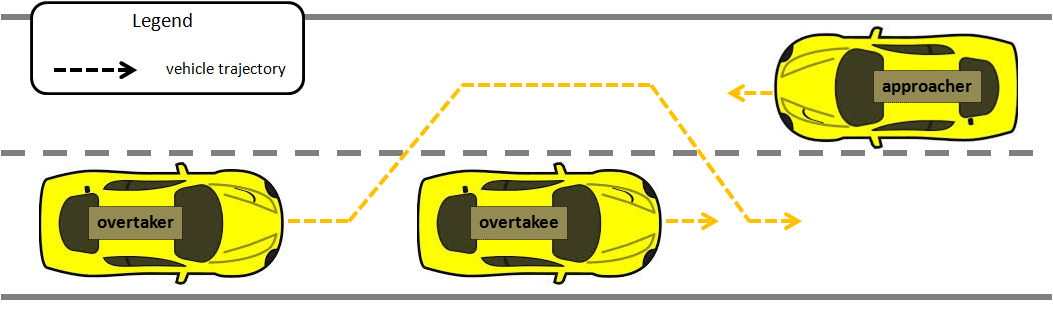
\includegraphics[width=\textwidth]{figures/overtakingWithApproacher.png}
\caption{Scenario}
\label{fig:scenario}
\end{figure}

In this scenario, there are three vehicles driving in two-lane road. Figure \ref{fig:scenario} shows the road and the three vehicles. Two vehicles drive one after another in one direction, while the third vehicle drives on the other lane in the opposite direction. The first two vehicles are named \textit{Overtaker} and \textit{Overtakee}. The third vehicle is named \textit{Approacher}. 

The \textit{Overtaker} wants to overtake the \textit{Overtakee} in a safe manner. This means that the \textit{Approacher} should be far enough during the overtaking. Otherwise, the overtaking should not be allowed. The vehicles can exchange messages in order to assure the safety in this scenario.  

  
\chapter{Basic requirements}
\label{chap-basic-2}

The scenario from Chapter \ref{chap-scenario-1} is modelled in \muml. From the model, we generate C code and deploy it to LEGO mindstorm robots representing the vehicles. The following is a list of our basic requirements:

\begin{itemize}

\item The vehicles drive by following a black line representing one lane. Therefore, there are two black lines for the two lanes.
\item There are two modes of velocity for each vehicle: fast and slow. The mode changes periodically. 
\item The road is divided in seven sections. Each vehicle knows the section number of the section where it is driving at the moment. When it drives in new section, it informs the section control by sending a message.  
\item When the \textit{Overtaker} gets close to the \textit{Overtakee} it asks for permission for overtaking. The \textit{Overtakee} agrees if it is currently driving in slow mode.
\item The overtaking needs to be approved also by the section control which checks the position of each vehicle, and agrees on overtaking if the \textit{Approacher} is at least two sections away from the \textit{Overtakee}.   
\item The \textit{Overtaker} start the overtaking only if the \textit{Overtakee} and sections control approve the requests. 
\item If the request is not approved, the \textit{Overtaker} has to change to slow mode. When the distance increases it may send new request
\item During overtaking, the \textit{Overtakee} and the \textit{Approacher} drive in slow mode. 

\end{itemize}
\chapter{Advanced requirements}
\label{chap-optional-3}

Here, we list additional requirements which make the scenario more complicated. We define them as optional. 

\begin{itemize}

\item The vehicles should be able to detect any obstacle on the road and break when they get too close.  
\item There is only one type of vehicle. Each vehicle can be \textit{Overtaker}, \textit{Overtakee}, and \textit{Approacher} at any time. 
\item The road is circular. 
\item The velocity mode of each vehicle can be remotely managed. There is a user interface for this purpose.  

\end{itemize}

  




%\nocite{*} %uncomment if you want unreferenced sources to appear
\bibliographystyle{includes/splncs}
\bibliography{citations,../../02_seminar/seminartheses}{}

\end{document}
